%!TEX TS-program = pdflatex
%!TEX root = i3det-top.tex
%!TEX encoding = UTF-8 Unicode

\section{The Digital Optical Module}
\label{sec:dom}
\textsl{(Chris Wendt; 10 pages)}

\subsection{A Functional Description of the DOM}

\subsection{Mainboard}
Cite the DAQ article\cite{ICECUBE:DAQ}.

\subsection{The Photomultiplier}
Cite the PMT article\cite{ICECUBE:PMT}.

\subsection{High Voltage}

\subsection{Flasher Board}

\subsection{Pressure Housing and Optical Gel}

\subsection{Mu-metal Magnetic Shield}

\subsection{Cable Penetrator}

\subsection{Mechanical Mounting - Harness Assembly}

\subsection{Production and Testing}

\subsection{Calibration}

\subsubsection{DOMCal}

\subsubsection{Flasher Calibrations}

\subsection{Performance and Reliability}
We have over $N$ DOM years in ice.  What can be said about 
the reliability?  This section could be quite important.

\subsubsection{DOM Survivability}

\subsubsection{Electronic Gain Stability}

\subsubsection{Baseline Stability and Noise}

\subsubsection{PMT Gain and Discriminator}

\subsubsection{Optical Sensitivity Stability}

\subsubsection{Dark Noise}


Figure: rate vs time at several depths, some curves showing typical strings and other curves showing worst outliers


Figure: rate vs temperature, can again include separate curve(s) for outlier string(s) (use David H’s plot)

\begin{figure}
 \begin{minipage}[t]{0.45\linewidth}
 \centering
  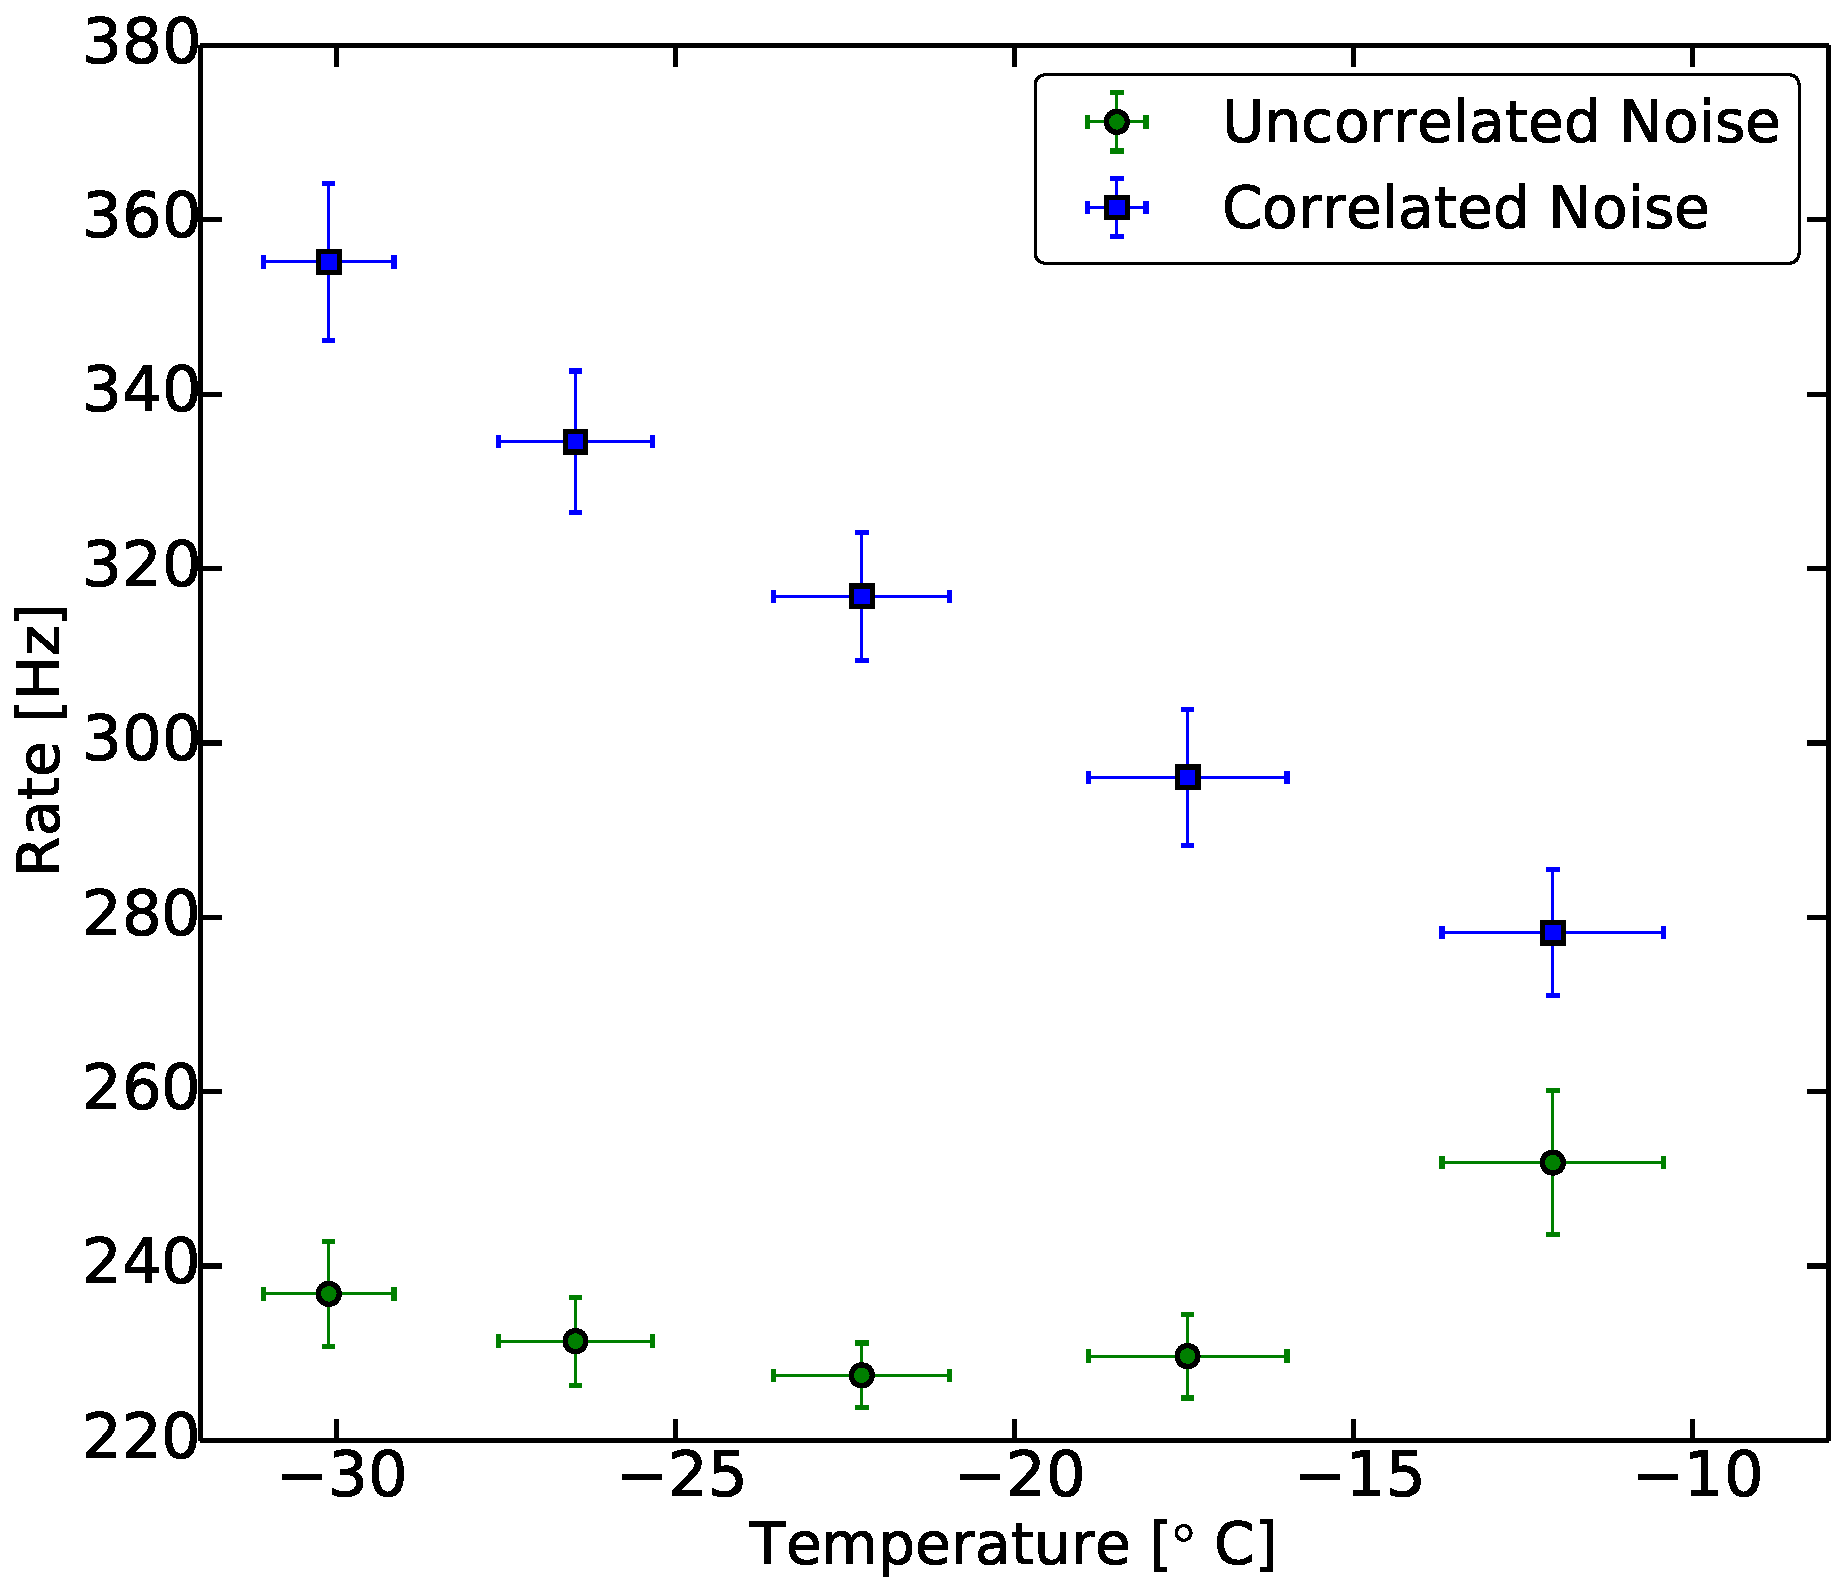
\includegraphics[width=\textwidth]{graphics/dom/performance/darknoise/HitRatevsTemp_inice_nomuons_nofit_bigfont.pdf}
 \caption{Noise rate in IceCube as a function of temperature, obtained from hitspooling data. Each data point represents the average of \num{12} DOM layers from \num{78} strings (DeepCore excluded). Atmospheric muon hits are subtracted.}
 \label{fig:HitRatevsTemp}
 \end{minipage}
\hfill
 \begin{minipage}[t]{0.45\linewidth}
 \centering
  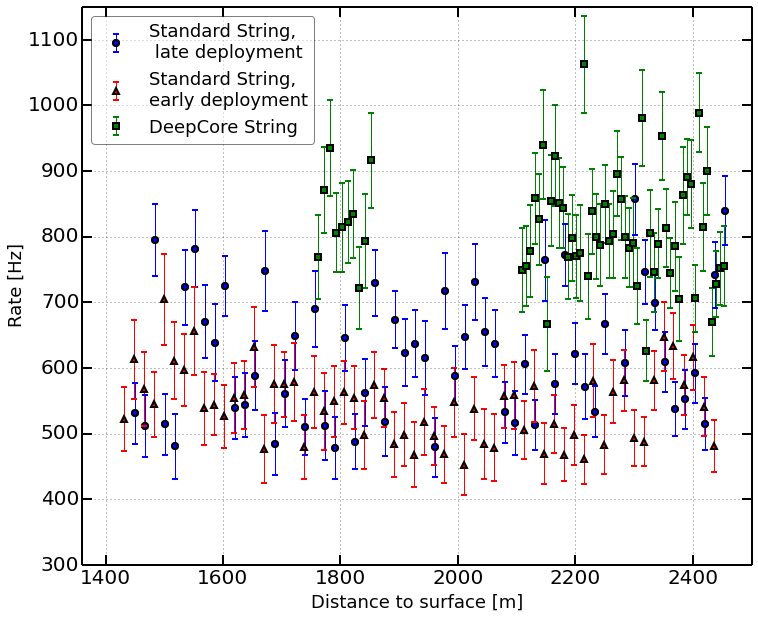
\includegraphics[width=\textwidth]{graphics/dom/performance/darknoise/StringHitRate_36_85.png}
 \caption{Hit rates per DOM for selected strings.}
 \label{fig:HitRatevsDepth_early_leate_dc_string}
 \end{minipage}
\end{figure}


time correlation important at low temp, explain counting with dead time (David H?)


experience with SHDR; one (?) DOM emitted flashes that could be seen on nearby DOMs, otherwise no impact from “flashing” PMTs affecting detector trigger; no bursts or dropouts of noise seen in SPE scalers, that would also be a way to see light-emitting discharge events in the same DOM where it occurred (need careful study of monitoring and/or SN data to prove that point); refer back to gain stability re smaller changes in noise rate
hitspooling studies (David H) if not elsewhere
